\documentclass[a4paper,12pt]{article}
\usepackage{amsmath}
\usepackage{tkz-euclide}
\usepackage{pgfplots}
\usepackage{mathtools}
\usepackage{multirow}
\usepackage{courier}
\usepackage{xcolor}
\usepackage{soul}
\usepackage{verbatim}
\usepackage{float}

\newenvironment{pseudocode}{\fontfamily{pcr}\selectfont}

\begin{document}
	\title{Title}
	
	\pagenumbering{arabic}
	\tableofcontents
	\newpage
	
	\section{Section 1}
	
	\subsection{Subsection 1}
	
	\noindent Simple array
	\begin{center}
		$\begin{array}{ccccc}
		1 & 0 & 0 & 0 & 1 \\
		0 & 0 & 0 & 0 & 0 \\
		0 & 0 & 0 & 0 & 0 \\
		0 & 0 & 0 & 0 & 0 \\
		1 & 0 & 0 & 0 & 1 
		\end{array}$
	\end{center}

	\noindent Displaying of items
	\begin{itemize}
		\setlength \itemsep{-0.5em}
		\item Item 1
		\color{red}
		\item Item 2
		\color{black}
		\item Item 3
		\begin{itemize}
			\item Subitem 1
			\item Subitem 2
		\end{itemize}
	\end{itemize}

	\noindent Enumeration
	\begin{enumerate}
		\item Item 1
		\item Item 2
		\item Item 3
	\end{enumerate}
	Different way to put an extra line: \textbackslash hfill \textbackslash break \\
	\hfill \break
	\noindent Table with caption
	\begin{table}[h]
		\caption{Title of table}
		\centering
		
		\begin{tabular}{| l | c | c | c | c | c |}
			\hline
			Item & 1 & 2 & 3 & 4 & 5 \\
			\hline
			Item & 2 & 3 & 3 & 4 & 5 \\
			\hline
			Item & 3 & 4 & 3 & 5 & 8 \\
			\hline
		\end{tabular}
	
	\end{table}

	\noindent Here table with no title and marked header and fixed length of columns.
	\begin{center}
		\begin{tabular}{ | p{0.2\linewidth} | p{0.15\linewidth} | p{0.17\linewidth} | p{0.48\linewidth} |}
			\hline
			Column 1 & Column 2 & Column 3 & Column 4 \\
			\hline \hline
			Value 1 & Value 2 & Value 3 & Value 4 \\
			\hline
			Value 1 & Value 2 & Value 3 & Value 4 \\
			\hline
		\end{tabular}
	\end{center}
	\hfill \break
	
	\noindent \newline Table with marged selected rows and columns 
	\begin{center}
		\begin{tabular}{| c | c | c | c |}
			\hline
			\multirow{4}{1em}{$\bigg\downarrow$} & 10 & 80 & 40 \\
			\cline{2-4}
			& 20 & 130 & 100 \\
			\cline{2-4}
			& 120 & 140 & 150 \\
			\cline{2-4}
			& 150 & 190 & 200 \\
			\hline
			\multicolumn{4}{|c|}{$\xrightarrow{\hspace{4em}}$} \\
			\hline
		\end{tabular}
	\end{center}
	
	\noindent \newline Using specially defined font for some part of text. \\
	\begin{pseudocode}
		IF weight(i) > j: M[i,j] := M[i-1,j]
	\end{pseudocode}
	
	\noindent \newline Few useful pictures: \\
	Graph with nodes and directed and non-directed edges
	\begin{center}
		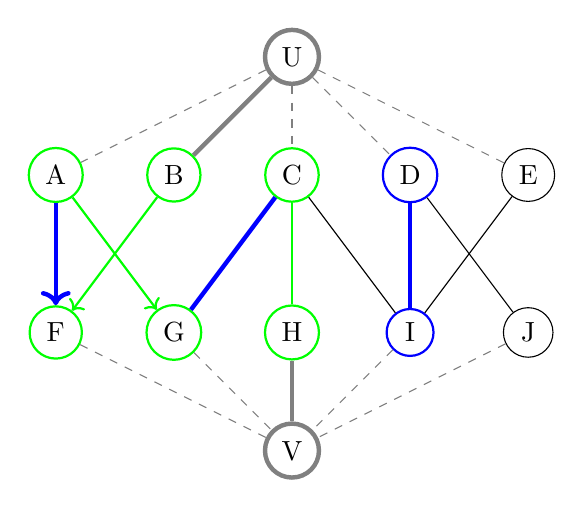
\begin{tikzpicture}
		\node[shape=circle,draw=gray, ultra thick] (U) at (0,1.5) {U};
		
		\node[shape=circle,draw=green, thick] (A) at (-3,0) {A};
		\node[shape=circle,draw=green, thick] (B) at (-1.5,0) {B};
		\node[shape=circle,draw=green, thick] (C) at (0,0) {C};	
		\node[shape=circle,draw=blue, thick] (D) at (1.5,0) {D};
		\node[shape=circle,draw=black] (E) at (3,0) {E};
		
		\node[shape=circle,draw=green, thick] (F) at (-3,-2) {F};
		\node[shape=circle,draw=green, thick] (G) at (-1.5,-2) {G};
		\node[shape=circle,draw=green, thick] (H) at (0,-2) {H};	
		\node[shape=circle,draw=blue, thick] (I) at (1.5,-2) {I};
		\node[shape=circle,draw=black] (J) at (3,-2) {J};
		
		\node[shape=circle,draw=gray, ultra thick] (V) at (0,-3.5) {V};
		
		
		\path [->, blue, ultra thick] (A) edge node[left] {} (F);
		\path [->, green, thick] (A) edge node[left] {} (G);
		\path [->, green, thick] (B) edge node[left] {} (F);
		\path [-, blue, ultra thick] (C) edge node[left] {} (G);
		\path [-, green, thick] (C) edge node[left] {} (H);
		\path [-] (C) edge node[left] {} (I);
		\path [-, blue, ultra thick] (D) edge node[left] {} (I);
		\path [-] (D) edge node[left] {} (J);
		\path [-] (E) edge node[left] {} (I);
		
		\path [dashed, gray] (U) edge node[left] {} (A);
		\path [-, gray, ultra thick] (U) edge node[left] {} (B);
		\path [dashed, gray] (U) edge node[left] {} (C);
		\path [dashed, gray] (U) edge node[left] {} (D);
		\path [dashed, gray] (U) edge node[left] {} (E);
		
		\path [dashed, gray] (F) edge node[left] {} (V);
		\path [dashed, gray] (G) edge node[left] {} (V);
		\path [-, gray, ultra thick] (H) edge node[left] {} (V);
		\path [dashed, gray] (I) edge node[left] {} (V);
		\path [dashed, gray] (J) edge node[left] {} (V);
		
		\end{tikzpicture}
	\end{center}

	\noindent Grid, with marked points and paths
	
	\begin{figure}[h!]
		\centering
		\begin{tikzpicture}
		\tkzInit[xmin=0, xmax=5,ymin=0,ymax=5]
		\tkzGrid
		\tkzDefSetOfPoints[prefix=P]{ 0/0, 0/4, 4/0, 4/4 }
		\tkzDrawPoints[fill=black](P1, P2, P3, P4)
		\node [above right, outer sep=2pt] at (4,4) {(4,4)};
		\node [above right, outer sep=2pt] at (0,0) {(0,0)};
		\node [above right, outer sep=2pt] at (0,4) {(0,4)};
		\node [above right, outer sep=2pt] at (4,0) {(4,0)};
		\draw [ultra thick,-] (0, 0) -- (0, 1) -- (1,1) -- (1,2) -- (2,2) -- (2,3) -- (3,3) -- (3,4) -- (4,4);
		\draw [ultra thick,blue,-] (0, 4) -- (0, 3) -- (1,3) -- (1,2) -- (2,2) -- (2,1) -- (3,1) -- (3,0) -- (4,0);
		
		\end{tikzpicture}
		\caption{Description of picture}
	\end{figure}
	

	\pagebreak
	\noindent Histogram with extra area marked
	\begin{center}	
		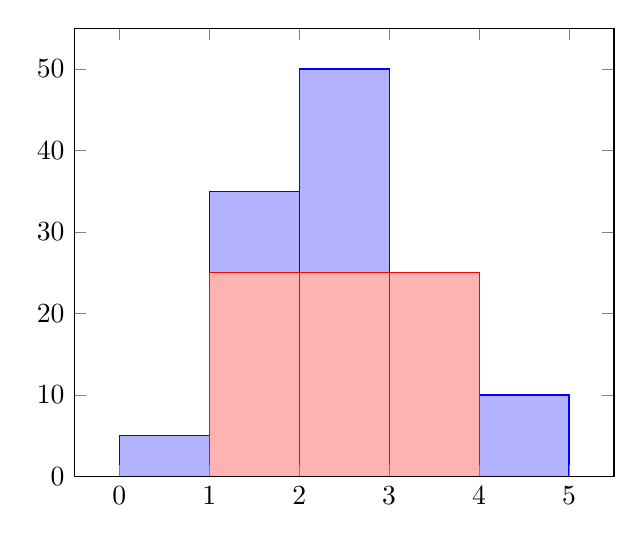
\begin{tikzpicture}
		\begin{axis}[ymin=0, ymax=55, area style]
		\addplot+[ybar interval,mark=no] plot coordinates {(0,5) (1,35) (2,50) (3,25) (4,10) (5,5) };
		
		\addplot+[ybar interval,mark=no] plot coordinates {(1,25) (2,25) (3,25) (4,25)};
		\end{axis}
		\end{tikzpicture}
	\end{center}

	\noindent Simple grid
	\begin{center}
		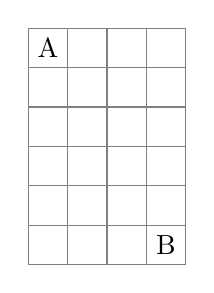
\begin{tikzpicture}
		\draw[step=0.5cm,color=gray] (-1,-1) grid (1,2);
		\node at (-0.75,+1.75) {A};
		\node at (+0.75,-0.75) {B};
		\end{tikzpicture}
	\end{center}

	\noindent Same grid with some colors:
	\begin{center}
		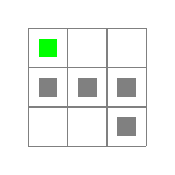
\begin{tikzpicture}
		\draw[step=0.5cm,color=gray] (-1,-1) grid (0.5,0.5);
		\node[fill=green] at (-0.75,+0.25) {};
		\node[fill=gray] at (-0.75,-0.25) {};
		\node[fill=gray] at (-0.25,-0.25) {};
		\node[fill=gray] at (+0.25,-0.25) {};
		\node[fill=gray] at (+0.25,-0.75) {};
		\end{tikzpicture}
	\end{center}
	
	
\end{document}
